\documentclass[border=2pt]{standalone}
\usepackage{tikz}

\tikzstyle{vertex}=[auto=left,circle,fill=black!25,minimum size=20pt,inner sep=0pt]

\begin{document}
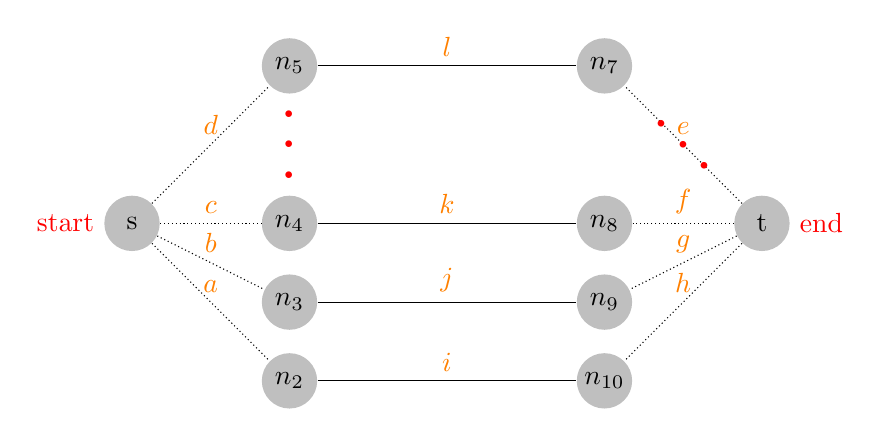
\begin{tikzpicture}
  \node[vertex] (n1)  at (1,4)  {s};
  \node[vertex] (n2)  at (3,2)  {$n_2$};
  \node[vertex] (n3)  at (3,3)  {$n_3$};
  \node[vertex] (n4)  at (3,4)  {$n_4$};
  \node[vertex] (n5)  at (3,6)  {$n_5$};
  \node[vertex] (n6)  at (9,4)  {t};
  \node[vertex] (n7)  at (7,6)  {$n_7$};
  \node[vertex] (n8)  at (7,4)  {$n_8$};
  \node[vertex] (n9)  at (7,3)  {$n_9$};
  \node[vertex] (n10) at (7,2)  {$n_{10}$};

  \foreach \from/\to/\weight in {n1/n2/a, n1/n3/b, n1/n4/c, n1/n5/d,
            n6/n7/e, n6/n8/f, n6/n9/g, n6/n10/h}
  \draw[densely dotted] (\from) -- (\to) node [midway, above, orange] {$\weight$};
  \foreach \from/\to/\weight in {n2/n10/i, n3/n9/j, n4/n8/k, n5/n7/l}
  \draw(\from) -- (\to) node [midway, above, orange] {$\weight$};;

  % These are for dotted lines
  %\draw [red, dotted, ultra thick] (n4) -- (n5);
  %\draw [blue,dotted, ultra thick] (n6) -- (n7);

  \path (n4) -- (n5) node [red, font=\Huge, midway, sloped] {$\dots$};
  \path (n6) -- (n7) node [red, font=\Huge, midway, sloped] {$\dots$};

  \node [left , red] at (n1.west) {start};
  \node [right, red] at (n6.east) {end};
\end{tikzpicture}
\end{document}